\chapter{Outline for a modernized Open Computer Forensics Architecture}
This appendix tries to show the big picture of a prospect computer forensics framework that builds on both the good parts of the Open Computer Forensics Architecture (OCFA), and the concepts and sub-systems introduced in the research paper. The idea of this appendix is to sketch a  the rough outlines of a possible OCFA inspired framework using modern day information technology components and insights gained from years of OCFA usage and the analysis done in Apendix-A. A framework that could fill the gap left by the discontinuation of OCFA development by the dutch police. While this gap has been filled successfully for dutch law enforcement by the non-open Xiraf framework developed by the Netherlands Forensic Institute, and while on a smaller scale the framework provided by PyFlag and more notably the Sleuthkit Hadoop Framework have taken interesting steps, Pyflag has not moved significantly beyond any of the poorer implementation choiches that OCFA made towards an architecture more in sync with modern distributed computing insights, while the Sleuthkit Hadoop Framework efforts, like OCFA seem to have been abandoned. Neither architectures have addressed the basics of disk-cache efficiency as addressed in this paper. Additionaly, neither have the two frameworks managed to provide the accademic community with a framework suitable for serious computer forensic research projects of the scale of for example the FIVES project that used OCFA at its core. While implementation of a full framework with the required properties fals far outside of the scope of a single MsC research project, this chapter will provide the architectural outline of such a framework and will explain how MatockFS would play a pivitol role in the realization of such a framework. We shall address the prospect Framework as \emph{Mattock}. The idea of the naming stems from the naming of the carving tool scalpel. The idea is that while a tool the size of and with the precission of a scalpel is indispensible at any scale, if you want to scale up your investigations to the scale of an archeological dig, you will need bigger tools like a mattock. Its just a working title for thye prospect architecture. Anyone picking up on this paper is invited to come up with a more suitable name for the resulting framework. 
\section{The OCFA architecture}
\begin{figure}
\centering
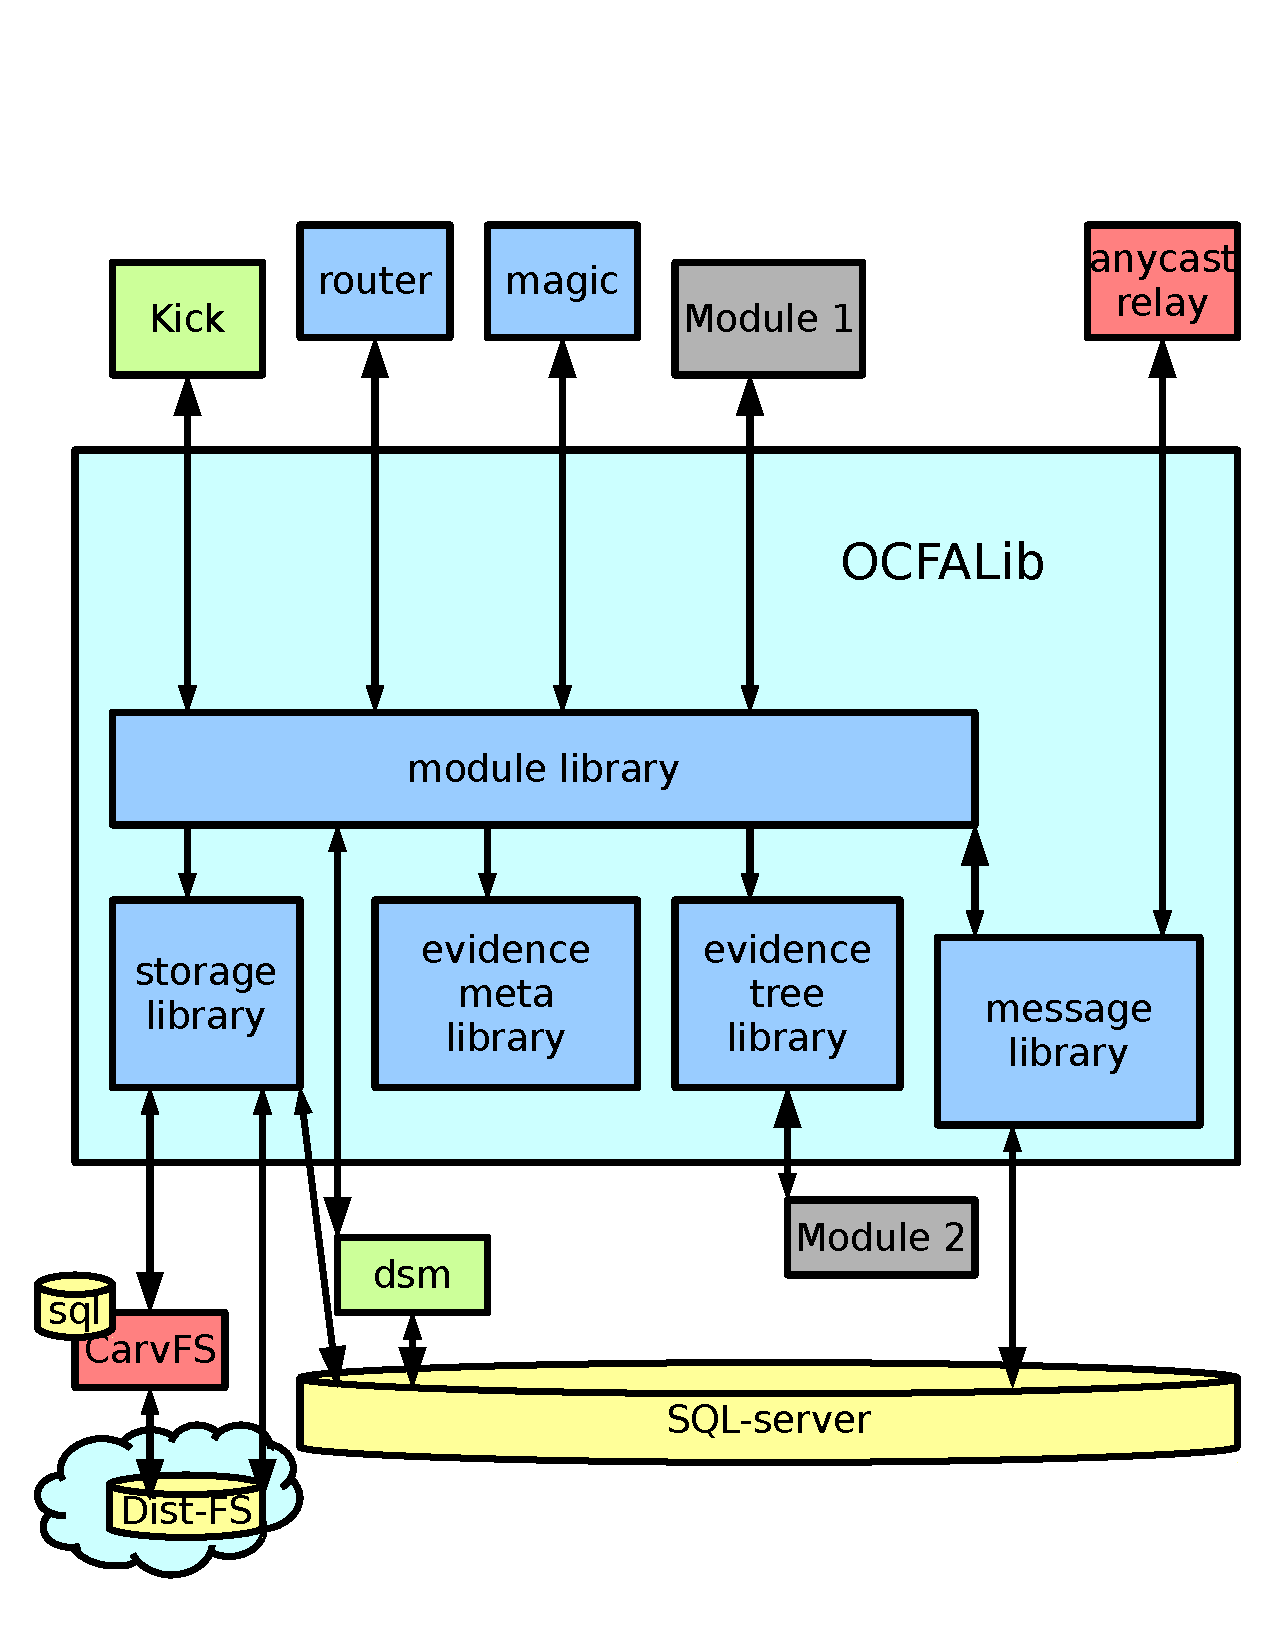
\includegraphics[width=100mm]{mattock/libraryview.pdf}
\caption{The base OCFA architecture}
\label{fig:FlowInOut}
\end{figure}
If we look at the OCFA architecture, at the core we basically see a fully custom build asynchonous messaging framework for processing modules that communicate with a small set of netwotrking components that act to combine the modules into dynamic chains of tools that are applied to parts of the forensic evidence data. The use of comodity software components is mostly limited to the pervasive use of XML technology and a central relational database. We shall have a look at some of the core components of the OCFA framework.
\subsection{The AnyCast Relay and Persistent Priority Queue}
At its basis, OCFA was a message passing concurency based system. One known issue with message passing concurency is the use of buffers. While message passing envinronemts like the Erlang programming language and platform opt to put producing processes to sleep when buffers fill up, OCFA opted for a different approach. In OCFA, the message passing buffers were managed by on-disk persistent priority queues. These queues only contained referenced to in database large text objects. The persistent queues were meant and designed to be fully crash resistent. The priority queus had a special \emph{'never'} priority to hold messages that were observed to crash specific modules. This allowed modules to be restarted and to skip problematic data untill a maintenance programmer would look at the problematic data and buggy module to fix the problem and re-submit the messages in the never queue for further processing. The Anycast relay was built on top of the persistent priority queue. Every module connected to the Anycast relay and registered as a consumer of a certain type (a module \emph{instance}) and would go into a message processing event loop asking the Anycast relay for new jobs. When a module was done with a peice of evidence data, or when a module derived a sub entity from such data (for example an attachment as child entity of an e-mail message), the module would send a message to the Anycast Relay adressed at a special process named the \emph{router}. The AnyCast would keep track of irresponsive and broken network connections and would play an important role in having stale or crashed modules restarted in a way not unlike what is common practice in Erlang based architectures. On such a detected crash, messages that were still pending a response would be put aside in the never queue to be looked at by a technision at a later point in time. In OCFA the AnyCast relay served as a single server for all modules, independent of the server these modules would run on.
\subsection{OcfaLib, a domain specific asynchonous framework}
While today NodeJS has mainstreamed the idea of a generic asynchonous framework, and while in other programming languages generic asynchonous frameworks such as Twisted for Python or Boost::asio for C++ have been available for quite a while, OCFA was first built long before such systems became mainstream. As a result, OCFA basically ended up building its own asynchonic processing framework. We could say that OcfaLib, the C++ OCFA library was a domain specific asynchonous framework for use with the AnyCast server. 
\subsection{The lagacy Module API}
OCFA came with two quite distinct module Application Programming Interfaces (APIs). This fact was the result of chronology of development. The first version of OCFA came with a module API not much unlike that of the current day sleuthkit framework. A module would get a file to process and could add meta data to that file, or, when it wanted to for example mark an extracted e-mail attachment as child entity, would submit that to the framework. The API consisted of a module initialisation part and a single method called 'processEvidence' that a module was supposed to overload. From within ProcessEvidence the module could either add meta or submit a child entity with added meta date.
\subsection{The Treegraph API}
After new modules got added to OCFA, the legacy module API was found to be lacking in the meta-data area. The problem was that a module deriving a tree of children would not be able to set meta-data for deeper child entities. Only level zero and level one meta data was possible. As a result, the more powerfull treegraph API was added. As porting old modules to the new API was considered a waste of precious development time, the old API was also still continued after the introduction of the new API.
\subsection{The legacy CAS storage}
OCFA in its initial release came with a Content Address Storage system for storing data entities. Data was created or, lacking CarvPath facilities, first coppied to a temporary file and hashed during copy. Once the hash was fully calculated, the temporary file was either moved to a location derived directly from the hash of its content, or discarded if an entity with the same hash was already pressent in the repository. 
\subsection{CarvFS}
Later releases of OCFA were made compatible with the use of CarvFS for parts of the storage needs. CarvFS integration has however remained a bit of a hack. The storage sub-system of OCFA used physical symbolic links to CarvFS CarvPaths inside of its primarily CAS based storage system. This meant that for example when using a CarvPath aware Sleutkit MMLS module, storage of a partition in the OCFA CAS storage system required the full partition to be read for hashing purposes before it could be symlinked in the storage subsystem.
\subsection{The meta-data based message router}
At the core of the OCFA architecture was the central meta-data based router. This XML technology based router would parse the meta-data that modules had gathered on a data entity and would based on an also XML-based rule-list determine the next hop in the tool-chain for that data entity. 
\subsection{The use of an SQL server}
There were two technologies that were pervasively used within OCFA. One XML we already discussed. The second one was a relational database. It was used by the storage subsystem, by the messaging subsystem, and finaly by the meta-data storing data-store-module. In each of these uses, the use of an SQL database turned out to be a sub-optimal choiche for a number of reasons. Some related to the creation of run-time performance bottlenecks and others related to the nature of the data structure and the nature of usefull analysis-time queries on this data. More on this when we discuss the alternatives for Mattock.
\section{PyFlag}
\begin{figure}
\centering
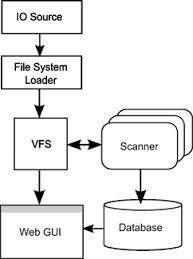
\includegraphics[width=50mm]{mattock/pyflag.jpg}
\caption{The base PyFlag architecture}
\label{fig:FlowInOut}
\end{figure}
Next to OCFA, the PyFlag framework deserves mention in this paper. While PyFlag has quite a different scope than OCFA it shares a lot of similarities too. Where OCFA is meant purely as a framework for computer forensics, PyFlag is a hybrid system that also addresses the field of network forensics. This hybrid approach makes that this framework would in a fundamental way be much more dificult to apply disk-cache related optimisations. It thus would be unfair to look at Pyflag purely from a large scale computer forensic data processing point of view in a comparitive way. 
\section{The Sleuthkit Hadoop framework}
A more promising development was the Sleuthkit Hadoop framework. It aimed to combine The Sleuthkit with specific distributed technology. The technology proposed was a combination of the HDFS distributed file-system and the distributed NoSQL database HBASE, both part of the Hadoop technology stack. These two technology choiches are absolutely takaway points we need to copy when implementing Mattock. That is, a distributed file-system and NoSQL technology. We shall look in more detail at suitable NoSQL technology. While HBASE isn't a bad choiche at the processing end, there are data structure and analysis concerns that would point to different NoSQL technology as potentially more suitable. 
\section{Non-open frameworks}
It is important to note that due to the closed nature of the frameworks involved, this paper does not look into some major and widely successfull non-open forensic frameworks such as Xiraff or FTK Distributed Install. The scope of this appendix is limited to open tools and publications.
\section{Digital Evidence Bags}
So far we have been looking purely at scalability and performance of forensic architectures without considering other important new computer forensic insights. One conceptual idea that all current frameworks seem to discard are the key concept introduced with so called Sealed Digital Evidence Bags (SDABs) by Bradley Schatz and Andrew Clark in 2006. While the details of SDABs fall outside of the scope of this appendix, one key aspect deserves special attention: The concept that both data and meta-data require a form of tamper-proofness. That is, once a piece of evidence data or meta-data is entered into the system, this (meta-)data should be considered to be logically immutable. We shall take this concept with us in our outlines for e next gereration scalable framework.
\section{New insights}
Looking back at OCFA and other forensic frameworks, there are in retrospect important suboptimal choiches that would be made differently if a framework like that was to be developed today. In this section we sumarize a few important insights that arose from years long usage of OCFA, a survey of other open frameworks. A literature survey and the results of the timing analysis in the first appendix of this paper.
\begin{itemize}
\item \emph{A treegraph API is essential} : While simpler API's can be usefull for some trivial modules, all such modules could also work with a more generic tree graph API. Having just one generic treegraph oriented API could facilitate a much wider range of modules and if the API is defined in asynchonous terms, the API could be portable to alternative architectures.
\item \emph{Leveraging asynchonous frameworks is essential} : OCFA implemented its own custom asynchonous framework and the part of the OCFA code-base involved with implementing that functionality was substantial. With current day asynchonous frameworks such as Boost::asio (C++), Twisted (Python) or NodeJS (JavaScript), the need for a custom built asynchonous framework has disapeared.
\item \emph{Evidence sealing facilities are a must} : It is esential to limit the mutability timespan and scope to an absolute minimum. Both from an anti-forensics point of view, and from the point of view of the legal credibility of the integrity of the implemented forensic process.
\item \emph{Reducing disk-cache misses is essential for performance}: While many papers focus on CPU cycles being wasted by inefficient forensic processes, the truth is that much of the forensic process is IO rather than CPU constrained. As such, the fact that the same data \emph{will} get read multiple times should make clear that a disk-cache miss will impact throughput and that a forensic framework such as OCFA with a design that does not effectively mittigate disk-cache miss rates will suffer from throughput disk-cache-miss related IO bottlenecks.
\item \emph{Zero-storage carving is esential} : The process of locating, carving and validating files on disk images is complex and will either result in high false positive or high false negative counts. In the case of high false-positives, copy-out will result in massive needs for forensic archiving storage for derived entities. In the case of high false negatives essential data may be missed. Applying zero-storage carving facilities such as CarvFS will allow for a relatively low cost of false positives while minimizing the amounth of aditional storage required for processing.
\item \emph{Simple priorities don't really work} : While our research has shown that priority queueing as used in OCFA would be effective for homogenously sized chunks of evidence data, not taking into account the size of the evidence entities and their likely disk-cache status in prioritizing has been shown to yield such poor results that the usefullness of priority queuing in such a way must be seriously questioned. 
\item \emph{Current day forensic disk image formats are poorely suited for large-scale processing archives} : In large scale investigations encompasing dozens to hundreds of full-size disk images, the in-lab usage of the common computer forensic disk image storage formats (EFF \& AFF) have shown to be rather poorly suited. Lacking a forensic lab storage format for large archives of disk images, the use of simple sparse dd images or basic directory tree with coppied out files as underlaying lab storage format seem to both be fastly better than. It would be ideal if future research would investigate the posibilities of archive friendly storage of computer forensic data.
\item \emph{Data migration should not be taken lightly} : While distributed file-systems or storage systems such as SNFS can facilitate in making evidence data available on many nodes, it is important to realize that accessing data from a different node will per definition result in a disk-cache miss on that node. It is suggested that data migration should prefer either the early out-of-cache migration of data that has not yet been fully cached by the originating module, or the migration of relatively small chunks of data targeted for relatively high-CPU processing on the other node. 
\item \emph{Relational (SQL) databases are a poor fit on all fronts} : In OCFA the Postgress SQL database was used for many things. In retrospect, certainly given the current day alternatives, these things would today all have better alternatives. First of all, the database usage for \emph{mutable} meta-data and for the storage and messaging subsystem together was a major performance bottleneck. Appart from the fact that in retrospect in-process mutable meta-data does not fit in with the SDEB view of things, a relational database is a poor choiche of technology for implementing either such metadata \emph{document} storage or the extra indirections implemented within the storage and messaging subsystems. More than that though, the usage of an SQL database by the data storage module and the user interface have shown that many of the more advanced analysises have had such shape and form that the database and queries would have been much better of having a more \emph{graph} oriented infrastructure. If we look at OCFA and than look at modern NoSQL technology, we see that parts of the SQL functionality had better be implemented without a database, ssome had better be implemented with a distributed \emph{key/value store} database, some with a \emph{document} database and some with a \emph{graph} database.  One thing all aspects of OCFA have in comon is that SQL technology in todays technology landscape would be a sub-optimal choiche at best. 
\item \emph{Kickstarting may not start at a server node} : In OCFA kickstarting took place from a server node. Before this could be done however, the EWF files had to be placed on an SNFS partition accessible to the server from a client through an SNFS connected file-server. Combine this with the need for converting EWF to dd or an other lab friendly format, the lack of a client-based EWF submitter led to massive disk write inefficiency. A kickstarting network client would need to be an essential component in a modern forensic framework.
\item \emph{Not all modules are alike} : All open forensic frameworks treat modules as equal citicens. The reality however is that some modules such as a file-type module are so common in data processing that framework embedding would be justified, some modules such as simple carvers are used mostly on huge data files and are IO intensive while others like OCR work on relatively small data chunks and take up significant CPU resources. Treating all modules and all data as similar will inevetably lead to poor overall framework performance. 
\item \emph{Globally valid annotations are the key} : As each server in a forensic data processing cluster has its own disk cache, the concept of dividing the load between different nodes by distributing and redistributing to different nodes should be possitively influencable by allowing nodes to have a common comunicatable notion of the portions of the global investigation data they and other nodes likely still have in their cache. For this, a globally valid annotation for data chunks is esential CarvPath annotations could play a major role in this.
\item \emph{Meta-data serialization technology matters} : At the time that OCFA was deviced, XML was the only logical choice for meta-data serialisation. The XML technology stack though is far from being the most efficient serialisation form for forensic meta data. While there are multiple papers proposing standarized XML formats for forensic meta-data exchange, the ineficciency of XML forms a major botleneck in event-rich high throughput processing such as in a computer forensic framework. More efficient serialisation options such as JSON, Protocol Buffers or Cap'n Proto should be seriously considered as alternative to XML. 
\item \emph{Hashing algorithm choiche is essential} :  Traditionally MD5 and later also SHA1 have been used as hashing algorithms in digital forensics. From a cryptographic pont of view, MD5 is now depricated while SHA1 is in the process of being depricated. Many public and law-enforcement-only hash collections like the Virusshare hash set or national child porography hash sets are still distributed only with MD5 and/or SHA1 hashes. Others like the NIST NSRL are now suplemented with SHA256 hashes. While the later may sound like good news, there is an other important issue with SHA256 for use in a forensic framework: SHA256 may be significantly more secure as a hashing algoritm than SHA1 or MD5, it is also significantly more CPU intensive. So much so that it may undermine the whole concept of opportunistic hashing as presented in this paper. While today NIST still considers the use of SHA1 for purposes as defined in this paper as \emph{acceptable use}, we must consider the retroactive impact that a cryptographer testifying on behalf of the defense and questioning the use of SHA1 in the forensic process may have a few years from now if SHA1 reaches the same level of deprication that MD5 has today. It thus can be argued that moving forward to a non-deprecated secure hasing algoritm should be considered a priority. Given the CPU resource issues with SHA256, it is also of paramount significance that the algoritm we move forwards to should have at least reasonable resource requirements in its software implementation. A quick study into available secure hashing algoritms reveals a small family of secure hashing algorithms. SKEIN, BLAKE and BLAKE2 share properties that would make each of these secure hashing algoritms prime candidates for suplementing and eventually replacing SHA1 as primary hashing algoritm for computer forensics. In the next appendix we will make the case for one of these. The important insight here however is the notion that SHA1 is close to deprication, SHA256 puts to much strains on resources in a high performance computer forensics setup and we need to pick a more suitable replacement.     
\end{itemize}
\section{A modernized OCFA inspired open-source architecture}
With the good parts from the old OCFA architecture combined with the new insights above, we can scetch the base outlines of a next generation message passing concurency open computer forensic framework. Let us start out with a rough description of the changes from the OCFA architecture to our new Mattock architecture outline. We see that the custom asynchonous framework gets replaced with boost::asio and twisted for the respective C++ and Python languages and that Python replaces Java as secondary platform language. We see that file-type logic and meta-data router are no longer a seperate module and network service but are now intergrated in the base functionality for each module process. Further we see the number of module APIs reduced to just the tree-graph API. The most obviously notable change however is the fact that there is no longer a direct dependency between generic modules and database technology. The SQL server has disapeared and has been replaced by other technology. The Data Store Module (DSM) maps the meta-data into a NoSQL database. This will most likely be a distributed graph-database or a distributed document-database (or possibly a hybrid combination of the two such as ArangoDb. Both data and now also meta-data are stored in a write-once way to the CarvFS replacement MattockFS that implements a subset of the SDEB concept by means of priviledge separation and immutability. The CarvFS longpath SQL database is replaced with a distributed key/value NoSQL database. While MattockFS should initially still run on SNFS or NFS, the use of a distributed file-system such as HDFS should be a potential way forward to further improve scalability. The Anycast Relay is replaced by a similar Anycast monitor meshup. One node per worker host. A Anyvast monitor will be a redesign of the Anycast that is fully CarvPath aware and is able to monitor a full worker host, both through the proc filesystem and through communication with MattockFS. The kickstarting process is revised. EWF processing is moved to the client side of things. The client connects to a central kick balancer that will query all anycast monitors to find the right kick server to redirect the client to. 
\begin{figure}
\centering
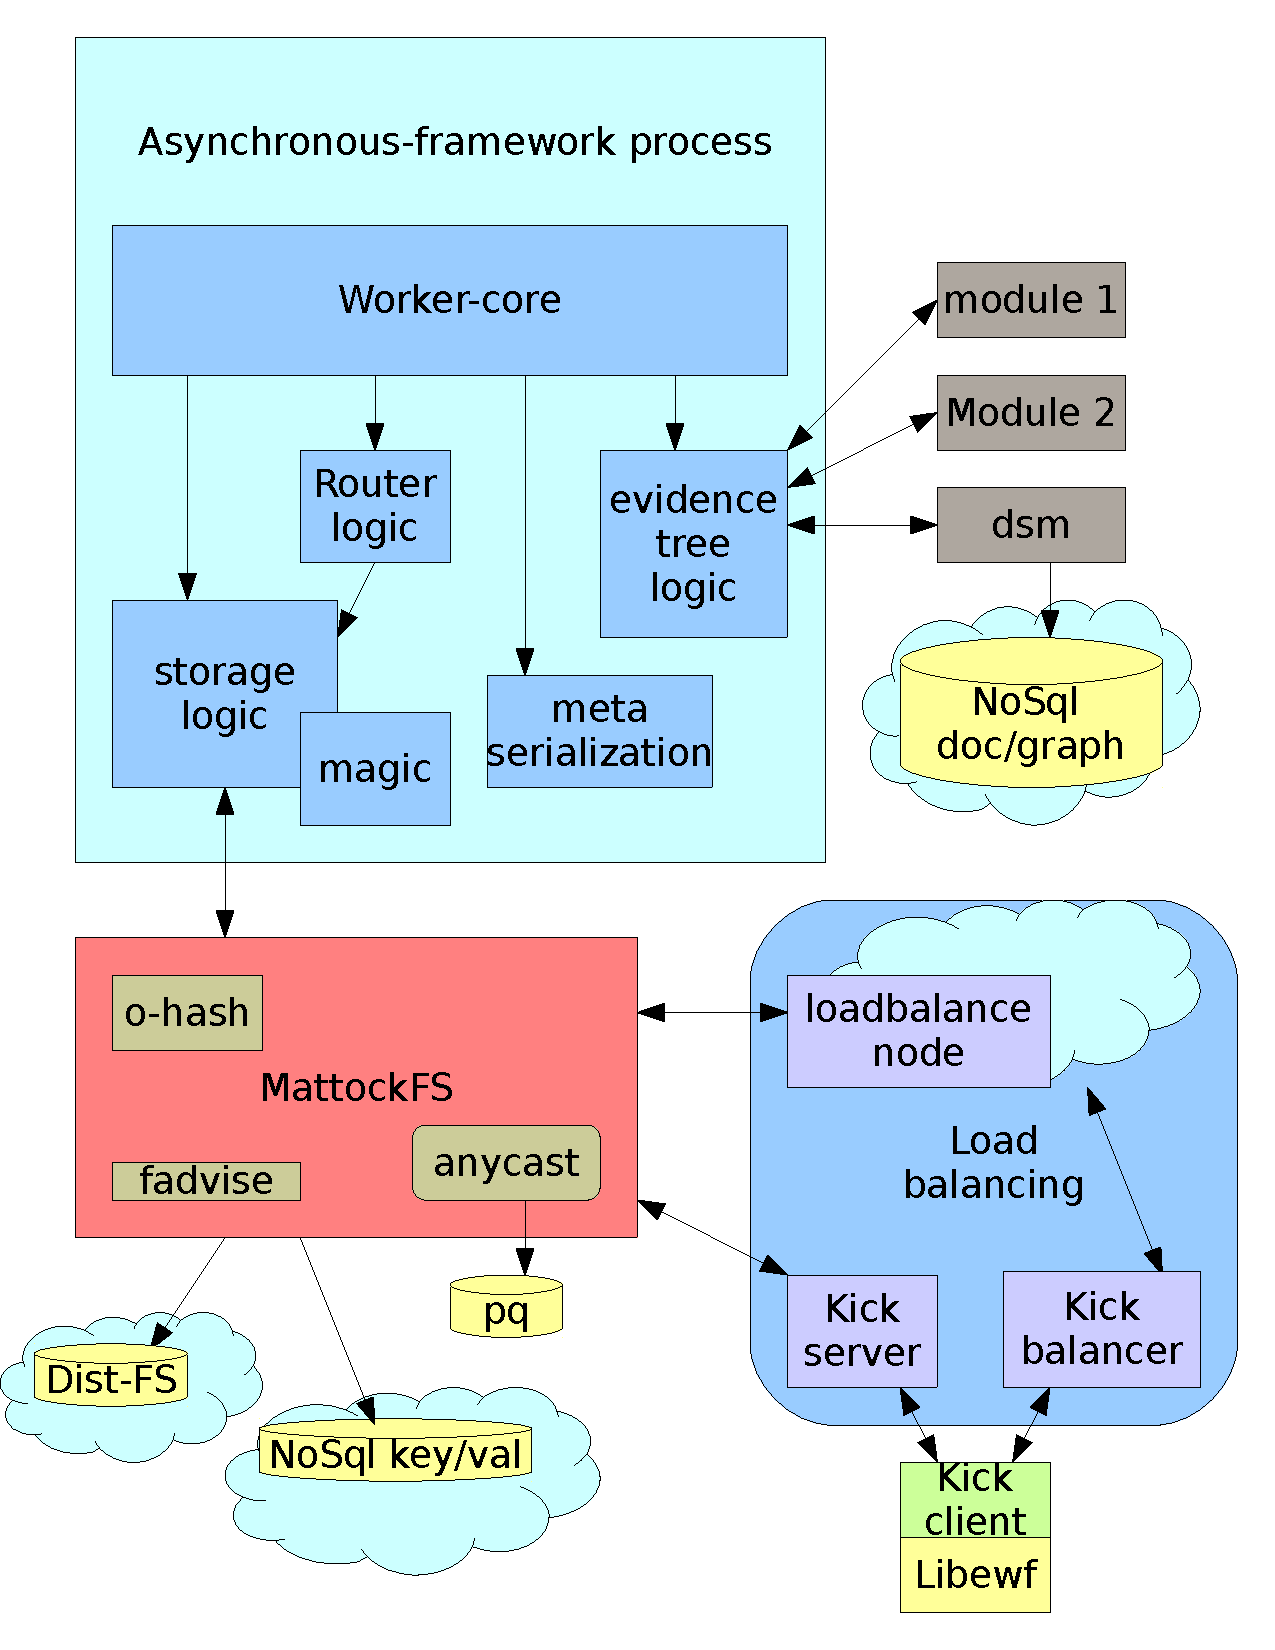
\includegraphics[width=100mm]{mattock/libraryviewmattock.pdf}
\caption{The base Mattock architecture}
\label{fig:FlowInOut}
\end{figure}
\subsection{The distributed longpath store}
\subsection{SNFS vs HFS}
\subsection{MattockFS \& the distributed longpath store}
\subsection{Effective distributed system usage}
\subsection{The AnyCast Monitor meshup}
\subsection{Client/Server kickstarting}
\subsection{Store-system embedded libmagic functionality}
\subsection{Distributed routing logic}
\subsection{From SQL to Graph based NoSQL}
\subsection{Using language-native asynchonous frameworks}
\subsection{A single tree-graph, lambda and asynchonous operation oriented API}
\subsection{Conclusion}
